


\chapter{Transport mésoscopique}

Nous allons dans ce chapitre aborder quelques notions de transport mésoscopique essentielles à la compréhension des résultats présentés dans la suite de cette thèse. La physique mésoscopique traite des systèmes de petites tailles, habituellement de la dizaine ou de la centaine de nanomètres~(parfois moins). Le transport mésoscopique s'intéresse plus particulièrement à la façon dons les électrons vont pouvoir circuler mais aussi interagir dans de telles structures pour donner naissance à des phénomènes quantiques tels que l'éffet Kondo ou le blocage de Coulomb. 

Il s'agit d'un domaine bien trop riche pour être traité dans un chapitre introductif et je concentrerai donc mon propos sur trois phénomènes déjà largement étudiés. Deux de ces phénomènes ont un point commun historique en cela qu'ils ont été découverts et expliqués bien avant la naissance de la physique mésoscopique telle que nous la connaissons aujourd'hui.

Le blocage de Coulomb par exemple que nous aborderons dans la première partie a été pour la première fois mis en évidence en 1951 par C.J. Gorter. Il avait constaté qu'en mesurant la conductance d'un matériau métallique granuleux à basse température, celle-ci diminuait de façon inattendue. Il expliquait cette baisse de conductance par la répulsion coulombienne au sein des grains de métal composant son matériaux. Nous montrerons comment ce phénomène joue un rôle central dans le transport à travers des structures mésoscopique.

L'effet Kondo que nous introduirons en fin de chapitre a lui aussi été mis en évidence dans la première partie du siècle dernier~(dans les années 1930) par des mesures sur un échantillon de métal massif contenant des impuretés magnétiques. Les mesures de conductances à basse température avait montré qu'après avoir atteint un maximum, la conductance diminuait à nouveau pour atteindre un valeur limite pour des températures proches du zéro absolu. L'explication du phénomène à tardé à venir et ce n'est qu'en 1964 que Jung Kondo a pu fournir une explication satisfaisante. Selon lui, les impuretés magnétiques agissent, à basse température, comme des centres diffuseurs très actifs diminuant d'autant la conductance de l'échantillon. Je donnerai plus de détails sur ce phénomène dans la suite du chapitre. En particulier, je détaillerai comment l'effet Kondo se manifeste dans les systèmes mésoscopiques.

Nous aborderons également un autre phénomène, le cotunneling, qui permet aux électrons de s'affranchir pendant un temps très court du régime de blocage de Coulomb. Nous verrons que ceci n'est possible que de part les lois de la physique quantique. Pour cela, nous distinguerons deux situation, l'une dans lequel aucun apport en énergie n'est nécessaire au phénomène - le cotunneling élastique- et une seconde pour laquelle if faudra fournir un certaine énergie au système - le cotunneling inélastique.

Nous préciserons pour chacun de ces phénomènes quantiques les conditions nécessaires (théoriques et expérimentales) à leur observation ainsi que les variables expérimentales dont ils dépendent.
%%%%%%%%%%%%%%%%%%%%%%%%
%SECTION I
%%%%%%%%%%%%%%%%%%%%%%%%


\section{Les paramètres du système}
Dans le cadre de nos expériences, nous avons utilisé ce que l'on appelle un transistor à électron unique ou Single Electron Transistor~(SET). En général un tel système est composé d'un point quantique~(ou ilôt) connecté à trois terminaux que l'on nommera source, drain et grille~(en référence aux transistors à effet de champ). L'il\^ot est couplé à ces trois terminaux par trois capacitances : $C_g$ pour la grille, $C_d$ pour le drain et $C_s$ pour la source. De plus, des barrière tunnel entre le point quantique et la source et le drain permettent le passage d'électron (sous certaines conditions) et sont caractérisées par les paramètre $\gamma_s$~(source/il\^ot) et $\gamma_d$~(drain/il\^ot). La source et le drain sont considérés comme des matériaux métalliques massifs et dont les électrons obéissent à la statistique de Fermi-Dirac. Enfin, nous attribuons à l'il\^ot une taille caractéristique $L$. 

Ce système, les paramètres qui le caractérisent ainsi qu'un schéma électrique équivalent sont représentés dans la Fig. \ref{description_systeme}. Nous allons maintenant détailler chacun de ces éléments.


\subsection{Les capacitances du système}
Comme expliqué précédemment, trois capacitances couples l'il\^ot central aux trois terminaux. L'application d'un tension sur l'un ou plusieurs de ces terminaux va donc modifier l'énergie du point quantique. Cette modification s'exprime comme suit :

\begin{eqnarray}
E = \frac{(C_sV_s + C_dV_d + C_gV_g)^2}{2(C_g + C_s + C_g)}=\frac{(C_sV_s + C_dV_d + C_gV_g)^2}{2C_{\Sigma}} \nonumber
\end{eqnarray}

Il est à noté que dans les expériences de Microscopie à Effet Tunnel ou Scanning Tunneling Microscopie~(STM), seules les tensions de source et de drain peuvent \^etre modifiées. Ce désavantage est compensé par la possibilité de modifier les paramètres de couplage $\gamma$~(que l'on détaillera dans la suite) en modulant la distance séparant la pointe de l'échantillon.

Ces capacitances vont également induire un "co\^ut" énergétique à l'ajout d'un électron dans l'il\^ot central. Cet ajout est associé à l'énergie $\frac{E_c}{2}$ appelé énergie de charge~(nous verrons l'utilité du facteur un-demi dans la suite ) dont la valeur est donnée par :
\begin{eqnarray}
\frac{E_c}{2} = \frac{e^2}{2(C_s+C_d+C_g)}=\frac{e^2}{2C_{\Sigma}} \nonumber
\end{eqnarray}


Cette énergie est à l'origine de la diminution de la conductance observée par C.J. Gorter en 1951. Lorsque la température est suffisamment élevée, elle fourni l'énergie nécessaire aux électrons pour passer d'un grain à l'autre. A basse température en revanche, les électrons n'ont plus la possibilité de se mouvoir de la sorte et la conductance mesurée diminue. On voit ici une première condition nécessaire à l'apparition du phénomène de blocage de Coulomb : $E_c \gg k_bT$.

En tenant compte de ces deux contributions, l'énergie d'un il\^ot contenant N électrons et soumis à trois tensions $V_g$, $V_d$ et $V_s$ est donnée par :
\begin{eqnarray}
U(N) = \frac{1}{2C_{\Sigma}} (-|e|N + C_sV_s + C_dV_d + C_gV_g)^2
\end{eqnarray}

On inclus parfois dans cette expression une charge $eN_0$ pour tenir compte de l'environement électrostatique. Nous verrons en abordant la notion de potentiel chimique que seule la différence d'énergie entre les différents états de charge importe et que donc l'offset introduit par ce dernier terme peut \^etre ignoré.

\begin{figure}
\includegraphics[scale=1]{Theorie/Transport/figure1/figure1ThTr.pdf} 
\caption{Paramètres caractérisant un système à trois terminaux}
\label{description_systeme}
\end{figure}



\subsection{L'il\^ot}
Les points quantiques que l'on utilise le plus fréquemment dans les expériences mésoscopiques sont souvent~(mais pas exclusivement) basés sur l'un des systèmes suivants:
\begin{itemize}
\item \textbf{un gaz d'électron bidimensionnel:} généralement une hétérostructre de semi-conducteur est utilisé pour obtenir un gaz d'électron bidimmensionnel proche de la surface. Par des technique de lithographie, des électrodes sont ajoutées sur la surface de l'échantillon. En appliquant une tension sur ces grilles, le gaz d'électron peut \^etre manipulé pour former un ou plusieurs points quantiques connectés à plusieurs électrodes.
\item \textbf{un grain métallique:} une grain de metal~(souvent noble) de quelques nanomètres joue le rôle de point quantique. Ces grains peuvent \^etre notamment obtenue en utilisant la technique d'électromigration que l'on verra dans la suite.
\item \textbf{une molécule:} c'est ce type de point quantique que nous utiliserons. Les molécule pouvant \^etre utilisées pour jouer ce r\^ole sont trop nombreuses pour toutes \^etre cité mais on peut néanmoins donner quelques exemples : les nanotubes, les fullerène, les aimants moléculaires etc.. \newline
\end{itemize}

Dans le cas d'électrons bidimensionnel ou celui d'un grain métallique, du fait de la taille des échantillons~($\sim 100nm$ pour les premiers, $\sim 10nm$ pour les seconds), on observe une quantification des différents états du système. Le spectre énergétique de l'il\^ot peut s'exprimer en fonction de trois nombres quantiques $n_x$, $n_y$ et $n_z$ à travers la relation suivante:
\begin{eqnarray}
E_n = \frac{\pi^2 \hbar^2}{2m}(\frac{n_x^2}{L_x^2} + \frac{n_y^2}{L_y^2} + \frac{n_z^2}{L_z^2}) \nonumber
\end{eqnarray}


Il s'agit bien entendu ici d'une expression très simplifiée car elle suppose une forme de potentiel de confinement difficile~(pour ne pas dire impossible) à obtenir en pratique (variation abrupte et hauteur de potentiel infini). Elle a le mérite en revanche de faire appara\^itre une deuxième condition nécessaire à l'observation de ce que l'on appelle habituellement le blocage de Coulomb quantique (par opposition au blocage de Coulomb classique où seul la quantification de la charge joue un rôle). En effet, pour résoudre le spectre de l'il\^ot, l'énergie associée à l'agitation thermique doit \^etre négligeable devant l'énergie séparant deux niveaux à savoir:

\begin{eqnarray}
\frac{\hbar^2}{2mL^2} \gg k_bT \nonumber
\end{eqnarray}

Si cette condition est facilement atteinte lorsque l'on utilise des gaz d'électrons bidimensionnels, elle est en revanche plus difficile à satisfaire dans le cas d'un point quantique métallique~(du fait d'une masse effective de l'électron très petite dans le premier cas contrairement au second). \newline


Lorsque des molécule sont utilisées, cette quantification apparait beaucoup plus naturellement à travers la notion d'orbitales moléculaires. En effet, c'est sur ces orbitales que vont venir s'ajouter les électrons lors de la charge de l'il\^ot. On peut donc venir sonder les différents niveaux d'énergie d'une molécule en étudiant les différentes énergies nécessaires à l'ajout d'un ou plusieurs électrons sur les différentes orbitales. On désigne souvent la dernière orbitale contenant un électron par HOMO~(Highest Occupied Molecular Orbital). De même, la première orbitale ne contenant aucun électron est désignée par le terme LUMO~(Lowest Unoccupied Molecular Orbital).

Il faut se garder cependant de penser qu'une molécule jouant le r\^ole de point quantique conserve les m\^eme propriétés qu'une molécule isolée. Tout d'abord, les niveaux d'énergie sont fortement influencés par la présence des électrodes du fait de l'hybridisation. De plus, la présence des électrodes peut induire une déformation qui va altérer la structure électronique de celle-ci. Ce phénomène est connu sour le nom d'effet Jhan-Teller. 

Nous montrerons par la suite que dans le cadre de l'électronique moléculaire et plus particulièrement celui de la spintronique moléculaire, il est important de pouvoir évaluer l'influence de ces différents phénomènes.

\subsection{Les paramètre de couplage tunnel $\gamma_{s/d}$}
On peut voir ces coefficient comme définissant "l'aisance" avec laquelle les électrons peuvent passer par effect tunnel de la source ou du drain vers l'il\^ot et vice-versas. Les valeur $\gamma_{s/d}$ sont déterminantes dans la valeur du courant qui va \^etre mesuré dans notre système. Plus précisément, de leurs valeurs va dépendre la conductance $G$ de l'échantillon. Partant de cette conductance, on peut par un raisonnement simple montrer que cette conductance doit \^etre telle que :
\begin{eqnarray}
G \ll G_0 \text{ avec } G_0 = \frac{2e^2}{h}
\end{eqnarray}
où $G$ est la conductance de l'échantillon et $G_0$ est le quantum de conductance ($\sim 77.5 \mu S$), $e$ est la charge de l'électron et $h$ la constante de Planck.


De plus, le paramètre $\gamma$ rend compte de l'hybridisation des niveaux d'énergie du point quantique avec ceux des électrodes. Cette hybridisation entraîne l'élargissement des niveaux d'énergie d'une largeur $\Delta E_{\text{intrinsèque}}$ donnée par :
\begin{eqnarray}
\Delta E_{\text{intrinsèque}} = h (\gamma_s + \gamma_d)
\end{eqnarray}

Cette élargissement est appelé élargissement intrinsèque par opposition à l'élargissement induit par la température. On peut deviner ici une seconde condition nécéssaire à l'apparition du phénomène de blocage de Coulomb à savoir $\Delta E_{\text{intrinsèque}} \ll E_c$. De plus, dans un régime de blocage fort on a $\Delta E_{\text{intrinsèque}} \ll k_bT$. Si cette dernière condition est remplie, on peut avoir accès par l'intermédiaire de des distribution de Fermi-Dirac des électrodes, à la température du système.




\section{La notion de potentiel chimique}
La notion de potentiel chimique est à mes yeux une des notions les plus importantes afin de comprendre de manière simple et intuitive le phénomène de blocage de Coulomb. Un exemple de son utilisation dans la cadre du transport quantique peut \^etre trouvé dans la très belle et très pédagogique revue de Hanson \textit{et Al.}. Dans cette section, nous allons tout d'abord présenter le concept de potentiel chimique. Nous exprimerons ensuite, à partir des considérations exposés dans la partie précédente, le potentiel chimique de la source, du drain et surtout de l'ilôt central.

\subsection{Définition}

On recontre souvent le potentiel chimique en thermodynamique lorsque l'on s'intéresse aux systèmes ouvert échangeant des particules~(cf. ensemble Grand Canonique). Cette grandeur défini la variation d'énergie d'un système d\^u à la modification du nombre de particules qui le compose. On le trouve parfois défini comme suit :
\begin{eqnarray}
\mu = \frac{\partial U}{\partial N} \nonumber
\end{eqnarray}
$U$ étant l'énergie du système et $N$ le nombre de particules. Dans la suite, nous allons plut\^ot adopter la notation de Hanson et Al. et prendre la définition suivante :
\begin{eqnarray}
\mu(N) = U(N) - U(N-1)
\end{eqnarray}
ou $\mu(N)$ est la modification en énergie apporté par l'ajout de la $N^\text{nième}$ particules, $U(N)$ et $U(N-1)$ étant respectivement l'énergie du système avec $N$ et $N-1$ particules.

\subsection{Expérience de pensé}

Partant de cette définition on peut imaginer un système de deux réservoirs contenant un grand nombre de particules, chacune d'entre elles possédant un potentiel chimique différent. Connectons les par un canal ne laissant passer qu'une particule de potentiel chimique $\mu_{canal}$. Si une particule du réservoir de droite possède le potentiel chimique $\mu_{canal}$, elle peut donc passer dans le réservoir de gauche. La particule passe tout d'abord du réservoir de droite au canal ce qui n'entra\^ine pas de variation dans l'énergie du système~($\Delta E = -\mu_{canal} + \mu_{canal} = 0$). De m\^eme, la particule peut ensuite passer du canal au réservoir de gauche. Les trois configurations : particule dans le réservoir de droite, de gauche ou dans le canal sont dégénérés et la particule peut circuler librement dans le système.

Supposons maintenant que le nombre de particules au potentiel chimique $\mu_{canal}$ soit plus grand dans le réservoir de droite que dans le réservoir de gauche. M\^eme si les particules de gauche peuvent circuler en direction du réservoir de droite, il y aura en proportion, plus de particules venant du réservoir de droite vers le réservoir de gauche. Il y a donc un flux moyen de particules de la droite vers la gauche. Au bout d'un temps plus ou moins long, le système devrait tendre vers un équilibre et le flux vers zéro. En revanche, si l'on maintient "artificiellement" cette différence en nombre de particules, le flux devrait perdurer.

Dans le cadre de notre nanostructure, les particules sont des électrons, le nombre de particule au potentiel $\mu$ est gouverné par la distribution de Fermi pondéré par la densité d'état. Le canal filtrant n'est rien d'autre que notre point quantique. En introduisant un tension source drain, on induit une différence entre la source et le drain dans le nombre d'électron possédant le bon potentiel chimique (i.e le potentiel chimique de l'\^ilot central). Un courant peut donc \^etre mesuré. Si l'on s'en tient à ce raisonement fort simple, ce courant devrait \^etre proportionnel à cette différence dans le nombre de particule, autrement dit, directement lié à la tension source drain.

Ce raisonnement certe un peu simpliste peut \^etre formalisé aisément dans le cadre de la méthode des équations pilotes. Il faudra pour cela tenir compte du fait que pour qu'un électron de potentiel $\mu$ passe par exemple de l'électrode droite à l'électrode gauche, il faut non seulement qu'il soit présent à droite mais aussi qu'il y ait un état disponible de m\^eme potentiel chimique à gauche. L'ensemble de la procédure à suivre est détaillé dans l'annexe?!.



\subsection{Les potentiels chimique de la source et du drain.}
L'expression du potentiel chimique de la source et du drain est directement donnée par $\mu_i = e V_i$ ou $i=source/drain$. Il s'agit en fait du niveau de Fermi des électrons dans la source et le drain (à ne pas confondre avec l'énergie de Fermi). Si l'on veut maintenant savoir quel est la probabilité dans un métal de niveau de fermi $\mu_F$ de trouvé un électron de potentiel chimique $\mu$, je peux utiliser la distribution de fermi et cette probabilité est donc égale à :
\begin{eqnarray}
p(\mu) = \frac{1}{1 + \exp{(\frac{\mu - \mu_F}{k_bT})}} \nonumber
\end{eqnarray}
où $\mu$ est le potentiel chimique de l'électron, $\mu_F$ celui du métal, $k_b$ est la constante de Boltzmann et $T$ est la température du système. On obtient donc en fonction des tensions source et drain:
\begin{eqnarray}
p_i(\mu) = \frac{1}{1 + \exp{(\frac{\mu - eV_i}{k_bT})}}
\end{eqnarray}
ou $i$=source/drain, $V_i$ est la tension appliquée et $e$ la charge de l'électron. Comme nous l'avons vu dans notre expérience de pensé, cette notion est essentielle dans la détermination du courant qui traverse notre structure.

\begin{figure}
\centering 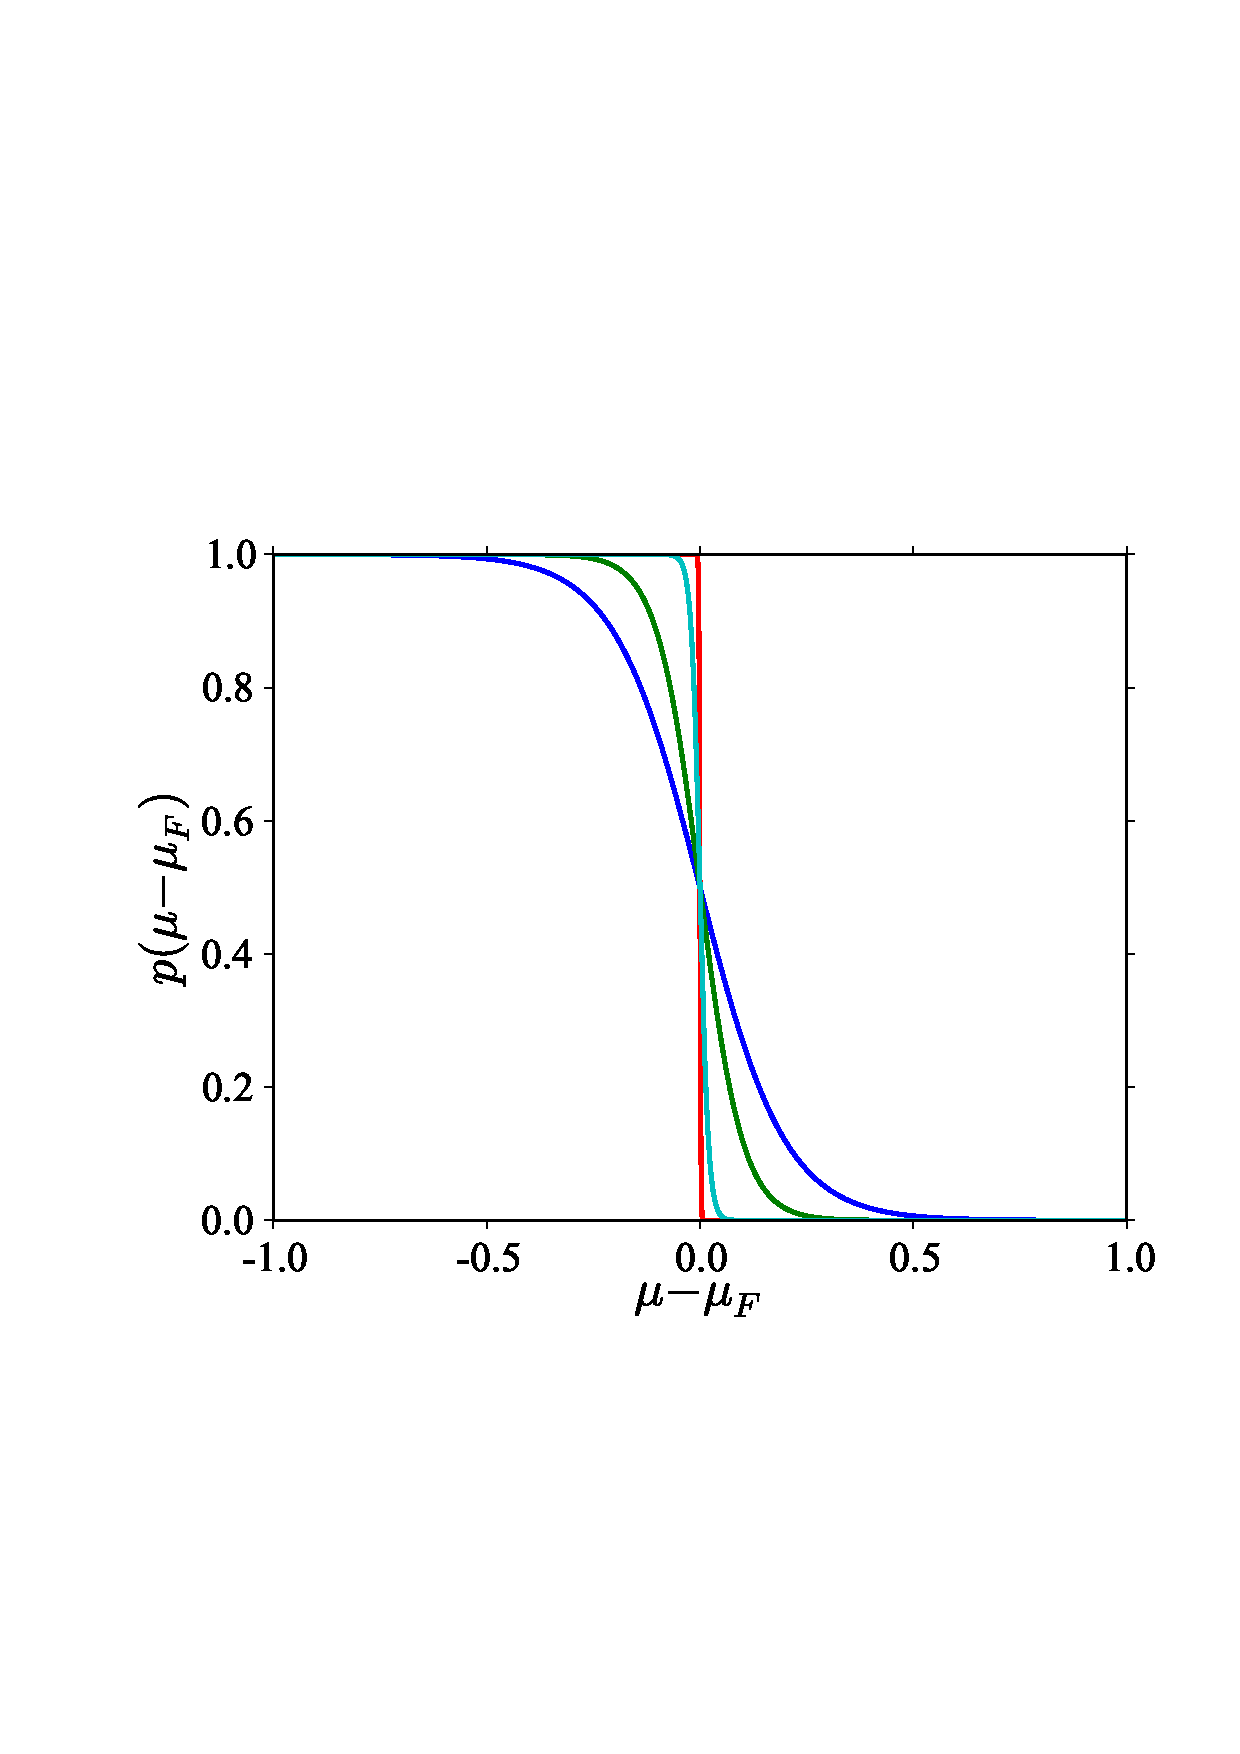
\includegraphics[scale=0.5]{Theorie/Transport/figure2/figure2.pdf} 
\caption{Probabilité d'avoir un électron de potentiel chimique $\mu$ sachant que le potentiel chimique du métal est $\mu_{\rm{F}}$. Le potentiel chimique $\mu_{\rm{F}}$ correspondant à une tension de $1mV$ que l'on applique habituellement dans ce genre d'éxpérience correspond à une énergie de $11.5K$.}
\label{distrib_fermi}
\end{figure}



\subsection{Le potentiel chimique de l'il\^ot}
Si l'expression du potentiel chimique de la source et du drain n'a rien de compliquée~(dans le cas d'électrode normale tout du moins), on ne peut pas en dire de m\^eme de celle de l'il\^ot. C'est m\^eme là que réside toute la difficulté de la compréhension d'une expérience. Heureusement, dans la partie précédente nous avons déjà fait le bilan des différentes énergie en jeux dans le système. A savoir, nous devons prendre en compte l'énergie électrostatique du système, l'énergie d'interaction électron-électron ainsi que la discrétisation des niveaux d'énergie dans l'il\^ot. Tout ceci donne :
\begin{eqnarray}
U(N) = \underbrace{\frac{1}{2C_{\Sigma}} (-|e|N + C_sV_s + C_dV_d + C_gV_g)^2}_{\text{couplage électrostatique et énergie de charge}}
+ 
\underbrace{\sum_{n=1}^{N} E_n}_{\substack{\text{énergie liés aux} \\\text{aux états discret}}}
\end{eqnarray}

On peut également tenir compte d'un éventuel champ magnétique en faisant le remplacement suivant :
\begin{eqnarray}
\sum_{n=1}^N E_n = \sum_{n=1}^N E_n(B) \nonumber
\end{eqnarray}
c'est à dire en attribuant à chaque niveau discret, une dépendance en champ magnétique. Nous verrons rapidement dans la suite comment cela se traduit dans le cas d'un système simple. 

Une fois l'énergie en fonction de $N$ exprimée simplement, il suffit d'appliquer la définition précédente à savoir :
\begin{eqnarray}
\mu(N) = U(N) - U(N-1) \nonumber
\end{eqnarray}

On se retrouve avec une expression relativement simple du potentiel chimique :
\begin{eqnarray}
\mu(N) = (N-\frac{1}{2})\frac{e^2}{C_{\Sigma}}
+ 
\frac{e}{C_{\Sigma}}(C_gV_g + C_sV_s + C_dV_d)
+
E_N(B)
\end{eqnarray}

En utilisant la définition de l'énergie de charge $E_c$ introduite précédemment, nous pouvons réécrire la relation sous la forme~(le terme 1/2 introduit précédemment permet une écriture plus compacte dans ce qui va suivre):

\begin{eqnarray}
\mu(N) = (N-\frac{1}{2})E_c
- 
\frac{E_c}{|e|}(C_gV_g + C_sV_s + C_dV_d)
+
E_N(B)
\label{pot_chim}
\end{eqnarray}

L'énergie $E_c$ est donc la quantité d'énergie d\^u à la répulsion Coulombienne qui sépare deux potentiels chimiques d'état de charge différents.


\section{Détermination des conditions de circulation d'un courant}
Pour rendre l'exposé qui va suivre plus clair, nous allons le décomposer en trois partie. Dans la première partie, nous allons voir quelles sont les conditions à remplir pour qu'un électron du drain puisse aller dans l'il\^ot. Dans la deuxième partie, nous ferrons de m\^eme pour la source. Enfin, dans la dernière partie, nous exploiterons les résultats obtenues pour en déduire les conditions nécessaires pour qu'un courant circule dans notre structure. Afin d'adapter les solutions trouvées aux conditions expérimentales, on posera $V_s = 0$ car dans la grande majorité des dispositifs, une des électrodes est directement connectée à la masse. Ce qui donnera $V_d=V_{ds}$, $V_{ds}$ étant la tension appliquée à l'échantillon.

\subsection{Charge de l'il\^ot par le drain}
Comme nous en avons discuté précédemment, pour qu'une particule (ici un électron) puisse passer d'un réservoir à l'autre, il faut que son potentiel chimique soit identique dans les deux réservoirs. Si l'on adapte se raisonnement à notre système, il faut donc qu'il y ait dans le drain des électrons dont le potentiel chimique corresponde à celui de cette électron une fois sur l'il\^ot. Supposons l'il\^ot dans l'état de charge $N-1$, pour passer à l'état de charge $N$, il faut qu'il y ait au moins un électron dans le drain dont le potentiel chimique soit égale à $\mu(N)$. Il nous suffit d'oberver la courbe de la Fig. \ref{distrib_fermi} pour comprendre que cela suppose :
\begin{eqnarray}
p(\mu) > 0 \Longrightarrow  -|e|V_{ds} \geq \mu(N) \nonumber
\end{eqnarray}

Ce qui conduit à la relation suivante :
\begin{eqnarray}
-|e|V_{ds} \geq (N-\frac{1}{2})\frac{e^2}{C_{\Sigma}}
-
\frac{|e|}{C_{\Sigma}}(C_gV_g + C_sV_s + C_dV_d)
+
E_N(B) \nonumber
\end{eqnarray}

En tenant compte des conditions $V_s= 0$ et que $V_{ds} = V_d$ évoquées plus haut, cette relation peut se réécrire de la façon suivante :
\begin{eqnarray}
V_{ds} \leq \frac{1}{C_g + C_s} \left\lbrace C_gV_g - \frac{C_{\Sigma}}{|e|}\left(E_N(B) + (N-\frac{1}{2})E_c \right) \right\rbrace 
\end{eqnarray}

La zone de transition entre charge et décharge dans le plan ($V_g$,$V_{ds}$) est délimité par une droite dont la pente $\dfrac{C_g}{C_g + C_s}$ est donnée par les différentes capacitances du système.


\begin{figure}
\includegraphics[scale=0.5]{Theorie/Transport/figure3/figure3.pdf} 
\caption{Représentation de la charge et de la décharge de l'il\^ot dans le plan ($V_g$,$V_{ds}$)}
\label{charge_discharge}
\end{figure}



\subsection{Charge de l'il\^ot par la source}
Un raisonnement similaire au précédent et en se rappelant que $V_s = 0$ conduit à la relation suivante :

\begin{eqnarray}
V_{ds} \geq -\frac{1}{C_d} \left\lbrace C_gV_g + \frac{C_{\Sigma}}{|e|}\left( E_N(B) + (N-\frac{1}{2})E_c \right) \right\rbrace
\end{eqnarray}


On peut extraire une deuxième pente $-\dfrac{C_g}{C_d}$ qui correspond à la charge ou la décharge de l'il\^ot par la source.

Nous pouvons également déduire de ce qui précède une deuxième relations importantes. Deux états de charge consécutifs sont séparés par une tension de grille $\Delta V_g$ que l'on peut relier aux paramètres du système par la formule suivante:
\begin{eqnarray}
\frac{C_g}{C_{\Sigma}} |e| \Delta V_g = E_c + \Delta E
\end{eqnarray}
où $\Delta E = E_N(B) - E_{N-1}(B)$ est l'écart entre deux niveaux d'énergie du spectre discret.
\subsection{Condition de circulation du courant}

Si l'on reprend les deux paragraphes précédents, on peut imaginer quatre situations :
\begin{itemize}
\item \textbf{Situation 1} : aucun électron ne peut \^etre chargé ni par la source ni par le drain. L'état de charge reste à N.
\item \textbf{Situation 2} : un électron peut \^etre chargé à la fois par la source et par le drain. L'état de charge est donc fixé à N+1.
\item \textbf{Situation 3} : un électron ne peut \^etre chargé que par la source. Dans ce cas, il finit par se décharger dans le drain
\item \textbf{Situation 4} : un électron ne peut \^etre chargé que par le drain. Dans ce cas, il finit par se décharger dans la source. \newline
\end{itemize}

Dans les situations un et deux, l'état de charge de l'il\^ot est bien défini et on se trouve dans le régime de blocage de Coulomb. Dans la situation 3 les électrons circulent de la source vers le drain. Un courant positif est donc mesuré. Dans la situation 4, les électrons circulent du drain vers la source. Un courant négatif est donc mesuré. L'emsemble de ces régimes est représenté dans la Fig. \ref{charge_discharge}.a. 

Souvent, les mesures ne se font non pas en courant mais en conductance différentielle $dI/dV$. Une simulation d'une telle mesure obtenue par la méthode des équations pilote est présenté dans la  Fig.\ref{charge_discharge}.b où les différentes zones décrites précédemment sont séparées par de grande variations dans la conductance différentielle mesurée.
\section{Etats excités et transport}

Dans de nombreux cas, une transition d'un état de charge à l'autre ne peut pas être associée à un unique potentiel chimique du fait de la présence d'état excité pour l'un ou les deux états de charges. Afin de décrire le transport dans ce cas précis, nous allons prendre un exemple simple d'une boite quantique oscillant entre les états de charges $N=0/1$. Nous tiendrons de plus compte du spin de l'électron. 

Sans champ magnétique appliqué le potentiel chimique $\mu_{+}$ associé à la transition d'un état de charge $N=0$ à un état de charge $N=1$ avec un état de spin up~($0\rightarrow +$) possède la m\^eme énergie que le potentiel chimique  $\mu_{-}$ associé la transition de l'état de charge $N=0$ à l'état de charge $N=1$ avec un état de spin down~($0\rightarrow -$).


Si l'on applique un champ magnétique au système, la dégénérescence en d'énergie des deux états de spin est levée du fait de l'effet Zeeman (cf Fig. \ref{charge_discharge}.b). Les deux potentiels chimiques $\mu_{-}$ et $\mu_{+}$ ne sont plus égaux. Le premier correspond désormais à la transition entre deux état fondamentaux~($EF(0)\rightarrow EF(1)$). Le second en revanche correspond à la transition de l'état fondamental $N=0$ à l'état excité de l'état de charge $N=1$~($EF(0)\rightarrow EE(1)$).

On peut donc construire deux jeux de diamant de Coulomb, l'un correspondant à $\mu_{-}$ et l'autre à $\mu_{+}$~(cf Fig. \ref{charge_discharge}.a en bleu et rouge respectivement). Cependant, dans les zones de blocage associé au diamant de la transition $EF(0)\rightarrow EF(1)$ (représenté ici par le potentiel chimique $\mu_{-}$) , aucun courant de peut circuler (zone grisé dans la Fig.\ref{charge_discharge}.a). Les bords de diamant situés dans cette zone doivent apparaître en pointillés car ils ne correspondent pas réellement à une modification du courant.

On voit que dans ce cas précis, un mesure en transport nous permet de mesurer directement le diagramme Zeeman, c.a.d la dépendence en champ magnétique des états du sytème. On peut donc utiliser cette technique pour effectuer une véritabel spectroscopie du point quantique. De plus, comme nous l'avons vu précédemment, les états de charge de l'il\^ot peuvant \^etre modifié à l'aide de la tension de grille. On peut donc chosir l'état de charge du système pour lequel on veut effectuer la spectroscopie.

 Bien s\^ur, il s'agit ici d'un système relativement simple et ceux rencontrer dans les expérience de transport sont parfois plus complexe. Ils arrivent souvent que les état N/N+1 possèdent tout deux des états fondamentaux et des états excités. Dans ce cas, l'analyse de la signature du système en transport devient plus difficile. Ces différentes configurations sont notamment traité par Hanson et Al., et un exemple peut \^etre trouvé dans l'analyse du $N@C_{60}$ proposé en fin de thèse et les références qu'il contient.

\begin{figure}
\includegraphics[scale=0.5]{Theorie/Transport/figure4/figure4.pdf} 
\caption{Diagramme Zeeman de l'état de charge N=1. Potentiel chimique correspondant à la transition 0/1}
\label{charge_discharge}
\end{figure}

\section{Cotunneling}
Nous avons vu jusqu'à maintenant que dans les zone de blocage de Coulomb, l'état de charge du système était fixe du fzit de l'énergie de charge. En effet, l'ajout d'un électron supplémentaire aurait un "co\^ut" énergétique trop grand pour le système. Cependant, l'on sait de part les inégalité d'Heinsenberg qu'un système peut outrepasser ce problème de "co\^ut" énergétique en "empruntant" l'énergie nécessaire pendant un temps très court. L'odre de grandeur de ce temps dépend de l'énergie nécessaire et est donnée par la relation :
\begin{eqnarray}
\tau \simeq \frac{\hbar}{E_c} \nonumber
\end{eqnarray}


\begin{figure}
\includegraphics[scale=0.5]{Theorie/Transport/figure5/figure5.pdf} 
\caption{Représentation du cotunneling dans le plan ($V_g$,$V_{ds}$)}
\label{charge_discharge}
\end{figure}


Un façon de voir le phénomène est de dire que pendant le temps $\tau$ un électron est entré dans le point quantique pendant qu'un autre en est sorti. Si un m\^eme état de charge possède plusieurs états~(fondamentaux et excités), on peut imaginer deux situations. Dans le premier cas, l'électron entrant vient occupé un état de m\^eme énergie que celui de l'électron sortant. On parle de cotunnling inélastique. L'électron entrant occupe un état d'énergie plus grand que l'électron sortant. On parle de cotunneling inélastique. Dans le deuxième cas, on comprend donc qu'il faut fournir cette différence en énergie à l'électron pour que ce type de cotunneling est lieu. Dans la suite, l'on notera cette différence d'énergie $\Delta E_{cot}$. Dans nos sytème, cette énergie est founis par la tension $V_{\rm{ds}}$. Pour qu'un processus inélastique est lieu, il faut donc que :
\begin{eqnarray}
|e|V_{\rm{ds}} \geq \Delta E_{cot}
\end{eqnarray}

On comprend donc que dans ce cas que le cotunneling élastique est toujour présent. C'est ce phénomène qui donne le fond de conductance mesuré dans les expériences de blocage de Coulomb. Plus intéressant encore, en faisant varier la tension de polarisation on peut venir sonder les différents état d'énergie pour un état de charge donnée. On peut donc effectuer une spectroscopie d'un point quantique en mesurant le cotunnling inélastique pour chacun

\section{Effet Kondo}

Tout comme le blocage de Coulomb, l'effet Kondo a d'abord été mesuré sur des échantillons macroscopique consistant en un metal massif contenant des impuretés magnétiques. En mesurant la conductance d'un tel échantillon à basse température, on avait constaté  qu'en dessous d'une certaine température la conductance avait tendance non plus a augmenté mais à atteindre un maximum pour diminuer à nouveau pour attendre une limite inférieure à celle attendu par les modèles de l'époque. Ce problème est resté insoluble pendant quelques années jusqu'au modèle proposé par Jung Kondo en 1964. Le modèle qu'il propose est relativement simple à concevoir mais en revanche très difficile à résoudre car faisant appel à la physique à $N$ corps. Dans ce modèle, les électrons de conduction viennent se coupler de façon antiférromagnétique aux impuretés magnétique du métal de telle sorte que le moment magnétique de l'impureté devient nul. Chaque impureté agit donc comme un centre de diffusion diminuant d'autant la conductance du système. La physique à $N$ corps apparait au travers des électrons de conduction. En effet, l'impureté magnétique n'interagit pas avec un seul électron du métal mais plutôt avec ce que l'on appelle un nuage Kondo. Il s'agit d'un phénomène hautement cohérent. Le seul problème du modèle à l'époque, c'est qu'il prevoit une divergence de la conductance quand la température tend vers zero. Il faudra attendre encore quelques année avec la théorie de renormalization proposé par Wilson, pour résoudre complètement le problème.

Ce problème est réapparu récemment dans ce que certain ont appelé "The revival of the Kondo Effect" (mettre la référence). La physique mésoscopique à permi de mettre à disposition des théoriciens des modèles beaucoup plus simple à résoudre dans lesquels le nombre d'inpureté magnétique pouvait être réduit à l'unité et également dans lequel le couplage aux électrons pouvait être contrôlé de manière précise. Les 2DEG par exemple permettent un contrôle quasi-parfait de ces différent paramètre. La littérature est riche en article et revues de toutes sortes couvrant de nombreux aspect de l'effet Kondo. Notre groupe à notablement contribuer à l'investigation de cette physique au travers notamment de l'étude de transition de phase et de Kondo sous écranté. Cependant, je ne traiterai pas en détail ici de ces effets là car je n'ai eu à utilisé l'effet Kondo que comme une sonde et non pas comme étude en soit. Je décrirai plus en détail dequelle manière nous avons procédé dans la partie réultats de cette thèse.

\begin{figure}
\includegraphics[scale=0.5]{Theorie/Transport/figure6/figure6.pdf} 
\caption{Kondo}
\label{Kondo_param}
\end{figure}


Je voudrait cependant dresser quelques généralités de l'effet Kondo dans les transistor moléculaire. Comme je le disait précedemment, l'effet Kondo~(de spin) réside dans le couplage anti-ferromagnétique entre une impureté magnétique et les électrons de conduction. Dans notre système, l'inpureté magnétique peut être joué par un niveau ne contenant qu'un seul électron non apparié. Il s'agit donc d'une impureté de spin $1/2$. Cette impureté est couplé aux électrons de la source et du drain. Première différence avec les systèles à base de 2DEG. Le couplage de l'impureté ne peux pas être contrôlé dans notre cas. Ce couplage anti-ferromagnétique n'est effectif qu'en dessous d'un température caractéristique nommé température Kondo et noté $T_K$ dans la suite. Cette température $T_K$ dépend principalement de trois paramètres : l'énergie de charge $E_c$, le couplage aux électrode $\gamma$ et la différence en énergie en entre le point quantique et le niveau de fermi des électrodes. Ces trois paramètre sont représenté sur la figure ??. La relation liant ces trois paramètre est la suivante:
\begin{eqnarray}
T_K \sim \frac{\sqrt{\gamma E_c}}{2} \exp(\frac{\pi \epsilon_0(\epsilon_0 + E_c)}{2\gamma E_c})
\end{eqnarray}
Première constatation, plus l'énergie de charge $E_c$ est grande plus la température Kondo sera élevé. C'est ici que réside un des avantages des transistors moléculaire comparitivement aux 2DEG. Les énergie de charge sont en général beaucoup plus élevé ce qui peut conduire à des $T_K$ de l'ordre de quelques dizaines de Kelvin. De plus, lorsqu'on s'éloigne d'un point de dégénéresence, $\epsilon_0$ augmente et donc la témpérature Kondo diminue pour atteindre son minimum au centre du diamant. On peut donc moduler $T_K$ par l'intermédiaire de la grille.